\documentclass[12pt,a4paper,oneside,ngerman]{article}
\usepackage[utf8]{inputenc}
\usepackage{color}
\usepackage{tikz}
\usetikzlibrary{arrows,shapes,automata,petri}
\usepackage{amsmath}
\usepackage{amssymb}
\usepackage{calc}
\usepackage{float}
\usepackage{listings}

\title{EZS}
\author{Simon Krücken}

\newcommand\tab[1][1cm]{\hspace*{#1}}

\begin{document}
    
\begin{titlepage}
%    \maketitle
\end{titlepage}
\tableofcontents

\section[Formeln]{Formeln}
Realzeitbedingungen:\\
\begin{itemize}
	\item 1. Realzeitbedingung:\\ \(\rho_{max,ges} = \displaystyle\sum_{j=1}^n \dfrac{t_{Emax,i}}{t_{Pin,i}} \leq c\) mit c = Anzahl Rechnerkerne
	\item 2. Realzeitbedingung: Für alle Rechenzeitanforderungen i muss gelten:\\ \( t_{Dmin,j} \leq t_{Rmin,j} \leq t_{Rmax,j} \leq t_{Dmax,j} \)
\end{itemize}

\(t_{Pmin,i} = minimal\) =$>$ \(t_{max,i} = \dfrac{1}{ t_{Pmin,i} }\) \\
\(t_{Pmax,i} = maximal\) \textcolor{gray}{$<$= uninteressant} \\
\(t_{Dmin,i}\) = minimal zulässige Reaktionszeit \\
\(t_{Dmax,i}\) = maximal zulässige Reaktionszeit

\begin{description}
    \item - Ausführuntgszeit (Executiontime) = Rechenzeit für eine RZ-Anforderung (ohne Warte oder Schlafzeiten)	
        \begin{description}
            \item - WCET \(t_{Emax,i}\) --$>$ Erfahrung oder Messen \textcolor{gray}{Worstcase}
            \item - BCET \(t_{Emin,i}\) = 0 \textcolor{gray}{Bestcase}
        \end{description}
    \end{description}

\(T_{Rmax,i}\) = maximale Reaktionszeit \\
\(T_{Rmin,i}\) = minimale Reaktionszeit \\
\(T_{R,i}\) = \textcolor{red}{\(t_{W,i}\)} \(+ t_{E,i}\) wobei \textcolor{red}{ \(t_{W,i}\) } Summe aller Wartezeiten

- Latenzzeit \(t_{L_i}\)
\textcolor{blue}{
	- Interrup Latenzzeit
	- Tasklatenzzeit
}

\(\rho_i = \dfrac{t_{E,i}}{t_{P,i}}\) Auslastung dur RZ-Anforderung i

\(\rho_{max,i} = \dfrac{t_{Emax,i}}{t_{Pin,i}}\) Worstcase, max. Auslastung

\fbox{
	\parbox{\textwidth}
	{
		1. RT Bedingung

		\(\rho_{max,ges} = \displaystyle\sum_{j=1}^n \dfrac{t_{Emax,i}}{t_{Pin,i}} \leq c\) \\
		j = für alle RZ-Anforderungen,
		c = Anzahl der Rechnerkerne
	}
}

\fbox{
	\parbox{\textwidth}
	{	
		\emph{Technischer prozess: }\\
		\begin{description}
			\item - \textcolor{blue}{\(t_{P,i}\)} = Prozesszeit, zeitlicher Abstand zwischen zwei RT-Anforderungen \textcolor{blue}{i} \fbox{ \textcolor{blue}{\(t_{Pmin,i}\)}}
			\item - \textcolor{blue}{\(t_{Dmin,i}\)} = minimal zulässige Reaktionszeit
			\item - \textcolor{blue}{\(t_{Dmax,i}\)} = maximal zulässige Reaktionszeit
			\item - \textcolor{blue}{\(t_{Ph,i}\)} = Phase, zeitlicher Abstand zwischen zwei \textcolor{red}{unterschiedlicher} Ereignise
		\end{description}
	}
}

\fbox{
	\parbox{\textwidth}
	{	
		\emph{Rechenprozesse: }\\
		\begin{description}
			\item - \textcolor{blue}{\(t_{Emin,i}\)} = minimale Ausführungszeit BCET
			\item - \textcolor{blue}{\(t_{Emax,i}\)} = maximale Ausführungszeit WCET
			\item - \textcolor{blue}{\(t_{Rmin,i}\)} = minimale Reaktionszeit
			\item - \textcolor{blue}{\(t_{Rmax,i}\)} = maximale Reaktionszeit\\ \rotatebox[origin=c]{180}{$\Lsh$} Zeitlicher Abstand zwischen dem Eintreffen einer RT-Anforderung \textcolor{blue}{i} und dem Ende der Bearbeitung
			\item - \textcolor{blue}{\(t_{W,i}\)} = Wartezeit, Summe der Zeiten, in der eine Codesequenz arbeiten könnte, aber nicht dran kommt.
		\end{description}
	}
}

\fbox{
	\parbox{\textwidth}
	{	
		\emph{Systemsoftware: }\\
		\begin{description}
			\item - \textcolor{blue}{\(t_{L,i}\)} = Latenzzeit, zeitlicher Abstand zwischen dem Eintreffen einer RT-Anforderung \textcolor{blue}{i} und dedm Start der Bearbeitung
			\item - \textcolor{blue}{Schedulingverfahren}
		\end{description}
	}
}

\fbox{
	\parbox{\textwidth}
	{
		1. RT Bedingung

		\(\rho_{max,ges} = \displaystyle\sum_{j=1}^n \dfrac{t_{Emax,j}}{t_{Pmin,j}} \leq c\) \\
		j = für alle RZ-Anforderungen,
		c = Anzahl der Rechnerkerne
	}
}

\fbox{
	\parbox{\textwidth}
	{
		2. RT Bedingung

		Für alle RZ-Anforderungen j muss gelten:

		\( t_{Dmin,j} \leq t_{Rmin,j} \leq t_{Rmax,j} \leq t_{Dmax,j} \)
	}
}

\fbox{
	\parbox{\textwidth}
	{
		Utilization
		\(u = \displaystyle\sum_{j=1}^n \dfrac{t_{Emax,j}}{ min(t_{Dmax,j}, t_{Pmin,j})} \)
	}
}

\section[Zeiten zeug]{Zeiten zeug}
\begin{lstlisting}
struct timespec {
        time_t   tv_sec;        /* seconds */
        long     tv_nsec;       /* nanoseconds */
};
\end{lstlisting}

\begin{itemize}
	\item CLOCK\_REALTIME\\ Systemweite realzeit Uhr. Diese Uhr zu setzten erfordert Root Rechte.
	\item CLOCK\_MONOTONIC\\ Kann nicht gesetzt werden. Gibt die vergangene Zeit ab einem unbestimmten Zeitpunkt an.
\end{itemize}

\begin{lstlisting}
#include <time.h>
main(int argc, char **argv)
{
	struct timespec start, end;
	clock_gettime(CLOCK_MONOTONIC, &start);	/* mark start time */
	sleep(1);	/* do stuff */
	clock_gettime(CLOCK_MONOTONIC, &end);	/* mark the end time */
	int diff = diff (end.tv_sec - start.tv_sec) + end.tv_nsec - start.tv_nsec;
}
\end{lstlisting}

\begin{itemize}
	\item Absolute Zeit: Zeit die überall gleich schnell ist
	\item Realtive Zeit: Zeit ist abhängig von der Geschwindigkeit und der Gravitation.
\end{itemize}

\begin{lstlisting}
#include <sys/time.h>

void timeradd(struct timeval *a, struct timeval *b, struct timeval *res);

void timersub(struct timeval *a, struct timeval *b,	struct timeval *res);

void timerclear(struct timeval *tvp);

int timerisset(struct timeval *tvp);

int timercmp(struct timeval *a, struct timeval *b, CMP);
\end{lstlisting}


\section[Petrie Netze]{Petrie Netze}
-$>$siehe Klausur
\section[Datenfluss Diagram]{Datenfluss Diagram}
-$>$siehe Klausur
\section[Struktugram]{Struktugram}
-$>$siehe Klausur
\section[Zeug]{Zeug}
\subsection{Harte und Weiche Realzeit}
Harte und weiche Realzeit/Echtzeit\\
\begin{figure}[H]
	\centering
	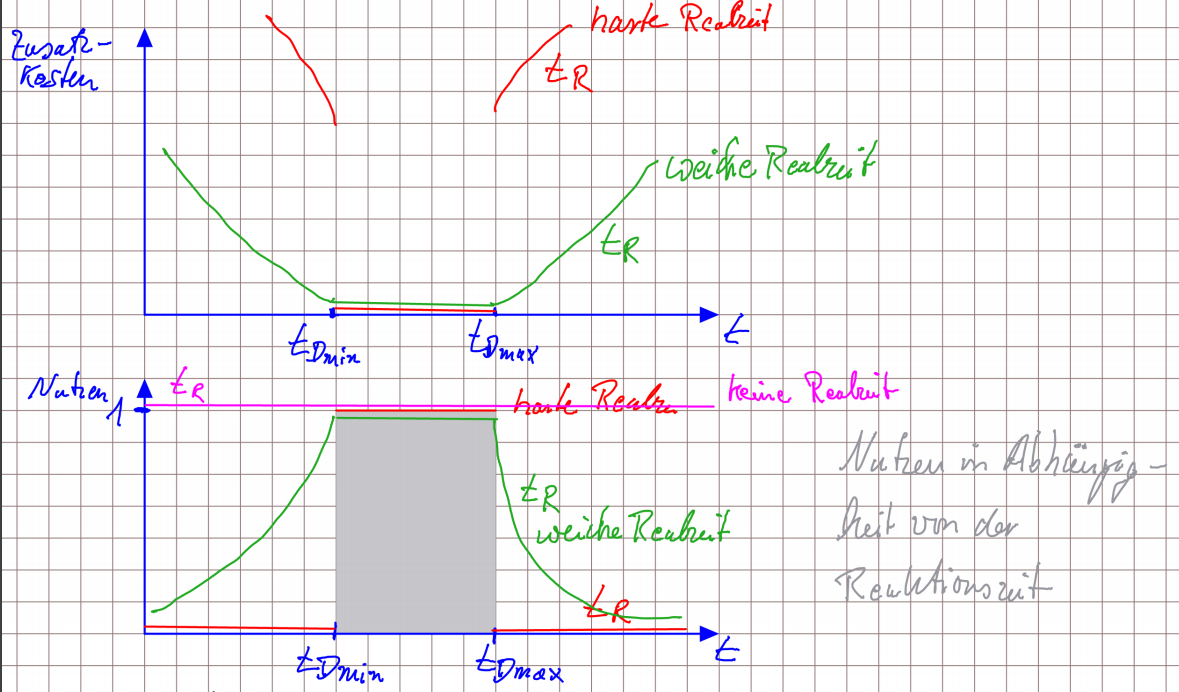
\includegraphics[scale=0.3]{umlet/harte_weiche_realzeit.png}
\end{figure}
\subsection{Bits}
Oberen 4 Bits von \textcolor{blue}{1010}1101 in Dezimal. \\
\textcolor{blue}{1010} allein stehen durch 4 mal bitshift rechts =$>$ 1010 = 0xA = 10

Bitsmaskieren:
\begin{itemize}
	\item AND 1010 \& 0111 = 0010
	\item OR 0101 $|$ 0011 = 0111
	\item XOR 0110 $\wedge$ 1011 = 1101
\end{itemize}

\section{Realzeitnachweise}
\subsection{Prioritätengesteuert}

\paragraph{1. Schritt:}
Anforderungen und zeitliche Parameter der Lösung zusammenstellen.
\paragraph{2. Schritt:}
Utilization überprüfen\\
\textcolor{blue}{Realzeitbedingungen werden grundsätzlich eingehalten, falls}\\

\textcolor{blue}{\(u \leq n\times( 2^\frac{1}{n} - 1)\) wobei n = Anzahl der Threads/Tasks, RT-Anforderungen}
\begin{description}
	\item \textcolor{magenta}{n = 1 =$>$ u \(\leq\) 100\%}
	\item \textcolor{magenta}{n = 2 =$>$ u \(\leq\) 82.8\%}
	\item \textcolor{magenta}{n = 3 =$>$ u \(\leq\) 78\%}
	\item \textcolor{magenta}{n -$>$ $\infty$ =$>$ u \(\leq\) 69.3\%}
\end{description}

\paragraph{3. Schritt:}
2. Realzeitbedingung überprüfen (falls u $\leq$ \textcolor{blue}{\(u \leq n\times( 2^\frac{1}{n} - 1)\))}\\
Problem: Bestimmung von \textcolor{blue}{\(t_{Rmax}\)} \\
Idee: Die \textcolor{blue}{\(t_{Emax}\)} der höhern oder gleich Prioren Tasks werden aufsummiert über die Zeit (= Arbeit für den Rechner zum Zeitpunkt t).
Es wird der Zeitpunkt gesucht, an dem die benötigte Zeit nicht mehr größer als die zur Verfügung gestellte Rechenzeit ist.\\

\( t_{c,p}(t) = \displaystyle\sum_{j \in J} \Big\lceil \dfrac{t}{ t_{Pmin,j} } \Big\rceil \times t_{Emax,j} \)\\
J = alle höher oder gleich Prioren Jobs\\
p = Priorität\\

Die zur Verfügung stehende Rechenzeit ergiebt sich zu \\
\textcolor{blue}{\( t_{available}(t) = t \)}\\
Gesucht ist damit die Lösung der Gleichung\\
\textcolor{blue}{\( t_c(t) = t \)}\\
Diese Gleichung lässt sich iterativ lösen:\\
Startwert: \textcolor{blue}{ \(t_{p}^{(1)<-Iterationsschritt} = \displaystyle\sum_{j \in J} t_{Emax,j} \)}\\

Iteration: \textcolor{blue}{ \( t_{p}^{(l+1)} = t_{c,p}(t_{p}^{(l)}) = \displaystyle\sum \Big\lceil \dfrac{t_{p}^{(l)}}{ t_{Pmin,j} } \Big\rceil \times t_{Emax,j} \) }

Abbruch: \textcolor{blue}{ \( t_{p}^{(l)} == t_{p}^{(l+1)} \) }  \textcolor{magenta}{ \( t_{Rmax,p} = t_{p}^{(l)} \) }

\pagebreak
\begin{table}[H]
	\caption{Beispiel:}
	\begin{tabular}{|l|l|l|l|l|l|l|l|l|l|}
	\hline
	RZ-Anf & \(t_{Pmin}\) & \(t_{Dmin}\) & \(t_{Dmax}\) & \(t_{Ph}\) & \(t_{Emin}\) & \(t_{Emax}\) & \(t_{Rmin}\) & \(t_{Rmax}\) & Prio \\ \hline
	A      & 30ms         & 0ms          & 20ms         & 0ms        & 2ms          & 10ms         & 2ms          &              & 1    \\ \hline
	B      & 45ms         & 0ms          & 45ms         & 0ms        & 3ms          & 15ms         & 3ms          &              & 2    \\ \hline
	C      & 60ms         & 0ms          & 60ms         & 0ms        & 4ms          & 15ms         & 4ms          &              & 3    \\ \hline
	\end{tabular}
\end{table}

\(t_{Emin}\) = \(t_{Rmin}\)\\

Berechnung der Utilization u:

\(u = \displaystyle\sum_{j=1}^n \dfrac{t_{Emax,j}}{ min(t_{Dmax,j}, t_{Pmin,j})}  =  \dfrac{10ms}{20ms} + \dfrac{15ms}{45ms} + \dfrac{15ms}{60ms} = 1.083 \)\\
\(\rho_{max,ges} = \displaystyle\sum_{j=1}^n \dfrac{t_{Emax,j}}{t_{Pmin,j}} \leq c => \dfrac{10ms}{30ms} + \dfrac{15ms}{45ms} + \dfrac{15ms}{60ms} = 0.917 \leq 1\)\\

Berechnung der Schranke für n = 3 \\
\(s = n\times( 2^\frac{1}{n}) = 0.78\)\\

Bedingung u $\leq$ 0.78 ist nicht erfüllt -$>$ weiter rechnen\\

\emph{Bestimmung von \(t_{Rmax,1}\) für die Jobs der Priorität 1}\\
1. Aufstellen von \( t_{c,p}(t) = \displaystyle\sum_{j \in J} \Big\lceil \dfrac{t}{ t_{Pmin,j} } \Big\rceil \times t_{Emax,j} \) = \( t_{c,1}(t) = \Big\lceil \dfrac{t}{ 30ms } \Big\rceil \times 10ms \)\\
2. Startwert: \( t_{1}^{(1)} = 10ms \) (= \(t_{Emax,1}\)) \\
3. Iteration: \( t_{1}^{(2)} = t_{c,1}(10ms) = \Big\lceil \dfrac{10ms}{30ms} \Big\rceil \times 10ms = 10ms\)\\
Abbruch, da: \( t_{1}^{(1)} == t_{1}^{(2)} \) =$>$ \( t_{Rmax,1} = 10ms \)\\

%\[\underbrace{VxWorks, Windows}_{\text{Round Robin}} \]

\emph{Priorität 2}\\
1. Aufstellen von \( t_{c,2}(t) =\) \(\underbrace{\Big\lceil \dfrac{t}{ 30ms } \Big\rceil \times 10ms }_{A} + \underbrace{\Big\lceil \dfrac{t}{ 45ms } \Big\rceil \times 15ms}_{B}\) \\
2. Startwert: \( t_{2}^{(1)} = t_{Emax,A} + t_{Emax,B} \) = 10ms + 15ms = 25ms \\
3. Iteration: \( t_{2}^{(2)} = t_{c,2}(25ms) = \Big\lceil \dfrac{25ms}{30ms} \Big\rceil \times 10ms + \Big\lceil \dfrac{25ms}{45ms} \Big\rceil \times 15ms = 25ms\)\\
Abbruch, da: \( t_{2}^{(1)} == t_{2}^{(2)} \) =$>$ \( t_{Rmax,2} = 25ms \)\\

\emph{Priorität 3}\\
1. Aufstellen von \( t_{c,3}(t) =\) \(\underbrace{\Big\lceil \dfrac{t}{ 30ms } \Big\rceil \times 10ms }_{A} + \underbrace{\Big\lceil \dfrac{t}{ 45ms } \Big\rceil \times 15ms}_{B} + \underbrace{\Big\lceil \dfrac{t}{ 60ms } \Big\rceil \times 15ms}_{C}\) \\
2. Startwert:\\ \( t_{3}^{(1)} = t_{Emax,A} + t_{Emax,B} + t_{Emax,C} \) = 10ms + 15ms + 15ms = 40ms \\
3. Iteration:\\ \( t_{3}^{(2)} = t_{c,3}(40ms) =\)\\ \tab \( \Big\lceil \dfrac{40ms}{30ms} \Big\rceil \times 10ms + \Big\lceil \dfrac{40ms}{45ms} \Big\rceil \times 15ms + \Big\lceil \dfrac{40ms}{60ms} \Big\rceil \times 15ms = 50ms\)\\
				\( t_{3}^{(3)} = t_{c,3}(50ms) =\)\\ \tab \( \Big\lceil \dfrac{50ms}{30ms} \Big\rceil \times 10ms + \Big\lceil \dfrac{50ms}{45ms} \Big\rceil \times 15ms + \Big\lceil \dfrac{50ms}{60ms} \Big\rceil \times 15ms = 65ms\)\\
				\( t_{3}^{(4)} = t_{c,3}(65ms) =\)\\ \tab \( \Big\lceil \dfrac{65ms}{30ms} \Big\rceil \times 10ms + \Big\lceil \dfrac{65ms}{45ms} \Big\rceil \times 15ms + \Big\lceil \dfrac{65ms}{60ms} \Big\rceil \times 15ms = 90ms\)\\
				\( t_{3}^{(5)} = t_{c,3}(90ms) =\)\\ \tab \( \Big\lceil \dfrac{90ms}{30ms} \Big\rceil \times 10ms + \Big\lceil \dfrac{90ms}{45ms} \Big\rceil \times 15ms + \Big\lceil \dfrac{90ms}{60ms} \Big\rceil \times 15ms = 90ms\)\\
Abbruch, da: \( t_{3}^{(4)} == t_{3}^{(5)} \) =$>$ \( t_{Rmax,3} = 90ms \)\\

\emph{Überprüfen der 2.RT-Bedingung}\\

\begin{table}[H]
	\begin{tabular}{lllll}
		   & \( t_{Dmin,j}\) & \(t_{Rmin,j}\) & \(t_{Rmax,j}\) & \(t_{Dmax,j}\) \\
	Prio 1 & 0ms $\leq$		 & 2ms $\leq$     & 10ms $\leq$    & 20ms          \\
	Prio 2 & 0ms $\leq$      & 3ms $\leq$     & 25ms $\leq$    & 45ms          \\
	Prio 3 & 0ms $\leq$      & 4ms $\leq$     & \textcolor{red}{90ms} $\leq$    & \textcolor{red}{60ms} \\
	\end{tabular}
\end{table}

Jobs der Priorität 3 (Task C) werden unter Umständen nicht schritthaltend abgearbeitet.\\



\pagebreak
\subsection{Deadline Scheduling}
\begin{table}[H]
	\caption{Beispiel:}
	\begin{tabular}{|l|l|l|l|l|l|l|l|l|l|}
	\hline
	RZ-Anf & \(t_{Pmin}\) & \(t_{Dmin}\) & \(t_{Dmax}\) & \(t_{Ph}\) & \(t_{Emin}\) & \(t_{Emax}\) & \(t_{Rmin}\) & \(t_{Rmax}\) & Prio \\ \hline
	A      & 30ms         & 0ms          & 20ms         & 0ms        & 2ms          & 10ms         & 2ms          &              & 1    \\ \hline
	B      & 45ms         & 0ms          & 45ms         & 0ms        & 3ms          & 15ms         & 3ms          &              & 2    \\ \hline
	C      & 60ms         & 0ms          & 60ms         & \textcolor{red}{10ms}       & 4ms          & 15ms         & 4ms          &              & 3    \\ \hline
	\end{tabular}
\end{table}

\paragraph{2. Schritt:} Auslastungsbedingung überprüfen\\
Grenze S = 1 $<$- auf Singelcore\\
\(\rho_{max,ges} = \displaystyle\sum_{i=1}^n \dfrac{t_{Emax,i}}{t_{Pmin,i}} \leq c => \dfrac{10ms}{30ms} + \dfrac{15ms}{45ms} + \dfrac{15ms}{60ms} = 0.917 \leq 1\)\\

\paragraph{3. Schritt:} Utilization überprüfen\\
\(u = \displaystyle\sum_{i=1}^n \dfrac{t_{Emax,i}}{ min(t_{Dmax,i}, t_{Pmin,i})} \leq 1 => \displaystyle\sum_{i=1}^n \dfrac{10}{20} + \dfrac{15}{45} + \dfrac{15}{60} = 1.083\) \\

weiterrechnen, da u $>$ s.\\

\paragraph{4. RT-Bedingung prüfen}:\\
\(t_{c}(I) = \displaystyle\sum_{i=1}^n \Big\lfloor \dfrac{I + t_{Pmin,i} - t_{Dmax,i} - t_{Ph,i} }{ t_{Pmin,i} } \Big\rfloor \times t_{Emax,i}\) \\
\(= \Big\lfloor \dfrac{I + 30ms - 20ms - 0ms }{ 30ms } \Big\rfloor \times 10ms\) \textcolor{blue}{A} \\
\(= \Big\lfloor \dfrac{I + 45ms - 45ms - 0ms }{ 45ms } \Big\rfloor \times 15ms\) \textcolor{blue}{B} \\
\(= \Big\lfloor \dfrac{I + 60ms - 60ms - 10ms }{ 60ms } \Big\rfloor \times 15ms\) \textcolor{blue}{C} \\
\(= \Big\lfloor \dfrac{I + 10ms }{ 30ms } \Big\rfloor \times 10ms + \Big\lfloor \dfrac{I}{ 45ms } \Big\rfloor \times 15ms + \Big\lfloor \dfrac{I - 10ms }{ 60ms } \Big\rfloor \times 15ms\)\\

\paragraph{5.}:\\
\( 0 \leq J kgV(30ms, 45ms, 60ms) + max(0ms, 0ms, 10ms) \) \\
\( 0 \leq J \leq 180ms + 10ms\)\\
\( 0 \leq J \leq 190ms\)\\

\paragraph{6.}:\\
Für Term \textcolor{blue}{A, B und C} alle J bestimmen damit Term Ganzzahlig wird. J muss unter 190ms bleiben.\\

\( \Big\lfloor \dfrac{I + 10ms }{ 30ms } \Big\rfloor = \) n für n = 1, 2, 3, ... \\
I = n * 30ms - 10ms für n = 1, 2, 3, ... \\
\( I_A = \{20ms, 50ms, 80ms, 110ms, 140ms, 170ms\} \)\\

\( \Big\lfloor \dfrac{I}{ 45ms } \Big\rfloor = \) n für n = 1, 2, 3, ... \\
I = n * 45ms für n = 1, 2, 3, ... \\
\( I_B = \{45ms, 90ms, 135ms, 180ms\} \)\\

\( \Big\lfloor \dfrac{I + 10ms }{ 60ms } \Big\rfloor = \) n für n = 1, 2, 3, ... \\
I = n * 60ms + 10ms für n = 1, 2, 3, ... \\
\( I_C = \{70ms, 130ms\} \)\\

\( 
	I_g = \{
	\underbrace{20}_{\text{+10}},
	\underbrace{45}_{\text{+15}},
	\underbrace{50}_{\text{+10}},
	\underbrace{70}_{\text{+15}},
	\underbrace{80}_{\text{+10}},
	\underbrace{90}_{\text{+15}},
	\underbrace{110}_{\text{+10}},
	\underbrace{130}_{\text{+15}},
	\underbrace{135}_{\text{+15}},
	\underbrace{140}_{\text{+10}},
	\underbrace{170}_{\text{+10}},
	\underbrace{180}_{\text{+15}} 
	\}
\)

\(
	t_c(20ms) = \Big\lfloor \dfrac{I + 10ms }{ 30ms } \Big\rfloor \times 10ms + \Big\lfloor \dfrac{I}{ 45ms } \Big\rfloor \times 15ms + \Big\lfloor \dfrac{I - 10ms }{ 60ms } \Big\rfloor \times 15ms\\
	= \Big\lfloor \dfrac{20ms + 10ms }{ 30ms } \Big\rfloor \times 10ms + \Big\lfloor \dfrac{20ms}{ 45ms } \Big\rfloor \times 15ms + \Big\lfloor \dfrac{20ms - 10ms }{ 60ms } \Big\rfloor \times 15ms\\
	= 10ms
\)

\(
	I \geq t_c(I)\\
	t_c(45ms) = 25ms \surd\\
	t_c(50ms) = 35ms \surd\\
	t_c(70ms) = 50ms \surd\\
	t_c(80ms) = 60ms \surd\\
	t_c(90ms) = 75ms \surd\\
	t_c(100ms) = 85ms \surd\\
	t_c(130ms) = 100ms \surd\\
	t_c(135ms) = 115ms \surd\\
	t_c(140ms) = 125ms \surd\\
	t_c(170ms) = 135ms \surd\\
	t_c(180ms) = 150ms \surd\\
\)

Überprüfen der unteren Schranken:


\begin{table}[H]
	\caption{Beispiel:}
	\begin{tabular}{lll}
	RZ-Anf & $t_{Dmin,i}$ & $t_{Rmin,i}$ \\ 
	A      & 0ms $\leq$   & 2ms $\surd$     \\ 
	B      & 0ms $\leq$   & 3ms $\surd$     \\ 
	C      & 0ms $\leq$   & 4ms $\surd$     \\ 
	\end{tabular}
\end{table}

Alle Bedingungen sind erfüllt. EDF klappt also.

\end{document}